\section{Introduction}
\label{chapter:Introduction}

Control-Flow Integrity (CFI)~\cite{abadi:cfi2, abadi:cfi} is one of the most used techniques to secure program execution 
flows against advanced Code-Reuse Attacks (CRAs). Advanced CRAs such as the recently published COOP~\cite{schuster:coop} 
and its extension~\cite{crane:readactor++} or the attacks described by the Control Flow Bending paper~\cite{carlini:bending}
are able to bypass most traditional CFI solutions, as they focus on indirect callsites, which are not as easy to determine at compile time.

This is a problem for applications written in C++, as one of its principle is inheritance and virtual functions. 
The concept of virtual functions allows the programmer to overwrite a virtual function of the base-class with his
own implementation. While this allows for much more flexible code, this flexibility is the reason COOP actually 
works. The problem is that in order to implement virtual functions, the compiler needs to generate a table of all
virtual functions for each class containing them and provide each instantiation of such a class with a pointer
to said table. COOP now leverages a memory corruption to inject their own object with a fake virtual pointer, 
which basically gives him control over the whole program, while the control flow still looks genuine, as no 
code was replaced. 

\textbf{Current solutions.} There exist several source code based solutions that either insert run-time checks during the compilation of 
the program like SafeDispatch~\cite{safedispatch:jang}, ShrinkWrap \cite{haller:shrinkwrap} or IFCC/VTV~\cite{vtv:tice}, 
which is the solution it is based on. Others modify and reorder the contents of the virtual table as their main 
aspect like the paper by Bounov et al.~\cite{bounov:interleaving}. While the recently published Redactor++~\cite{crane:readactor++}
implements a combination of those ideas.

While this might seem that only C++ is vulnerable, while C is safe, this notion is wrong, as the 
Control Flow Bending paper \cite{carlini:bending} proposes attacks on nginx leveraging global 
function pointers, which are used to provide configurable behavior.

As previously mentioned, there exist many solutions when one tries to tackle this problem while access
to the application in question is provided. However, when we are faced with proprietary third party 
binaries, which are provided as is and without the actual source code, the number of tools that can
protect against COOP or similar attacks is rather low.

\textbf{Limitations.} TypeArmor~\cite{veen:typearmor} implements a fine grained forward edge CFI 
policy based on parameter count for binaries. It calculates invariants for calltargets and indirect callsites based on
the number of parameters they use by leveraging static analysis of the binary, which then is
patched to enforce those invariants during run-time. The main shortcoming of TypeArmor is that
even with high precision in the classification of 
calltargets and callsites, one cannot exclude calltargets with lower parameter number from 
callsites, for one due compatibility and also due to variadic functions, which are a special
case in themselves. This basically means that when a callsite prepares 6 parameters, it is 
able to call all address taken functions. This generates a considerable attack surface due to the many
situations in which this policy can be naturally circumvented.

In this paper, we present \textsc{TypeShield}, a runtime illegitimate forward 
calls detection tool that can be seamlessly integrated with large scale applications such as web servers.
It takes the binary of an program as input and it can automatically instrument the binary in order
to detect illegitimate indirect calls at runtime. 
We implemented \textsc{TypeShield} to demonstrate a possible remedy of this problem by introducing
parameter types into the classification of callsites and calltargets. We explore to
what extent we can further narrow down the set of possible targets for indirect callsites
and manage to stop the exploitation at the binary level w.r.t. TypeArmor.
Our conclusion is that our tool can not stop all possible attacks since even solutions 
with access to source code are unable to protect against all possible attacks~\cite{carlini:bending}.
Nevertheless, we show that \textsc{TypeShield}, our binary based tool can stop all 
COOP attacks published to date and significantly raises the bar for an adversary when compared our tool with 
TypeArmor and other similar tools. 
Moreover, \textsc{TypeShield} provides strong mitigation for many types of code-reuse attacks
(CRAs) for program binaries, without the need for source code. 

\textbf{Our Insight.} \textsc{TypeShield} is based on a forward-edge CFI policy that 
relies on a precise construction of both the callee prototypes and callsite signatures
and than uses this information to enforce that each callsite targets matching functions 
only. For example, \textsc{TypeShield} disallows an indirect call that prepares
fewer arguments than the target callee consumes and where the types of the 
arguments provided are not super types of the arguments expected at the target.
Additionally, \textsc{TypeShield} incorporates an improved protection policy
which further reduces the possible target set of callees for each callsite.
Our novel policy is based on the insight that if the binary adhere to the standard calling convention
for indirect calls, undefined arguments at the callsite are not used by
any callee by design. \textsc{TypeShield} trashes these so-called
spurious arguments and thus breaks all published COOP
and improved COOP-like exploits. These exploits all chain
virtual method calls that disrespect calling conventions to
achieve convenient data flows between gadgets~\cite{crane:readactor++}.

Current binary based techniques enforce imprecise forward-edge CFI 
plocies, often allowing controll transfers from any valid callsite 
to any valid referenced entry point~\cite{ccfir:zhang, zhang:usenix}. 
In the best case, existing policies only reduce the target set by
removing all entry points of other modules unless they were
explicitly exported or observed at runtime~\cite{payer:dimva}. 
In contrast, \textsc{TypeShield} matches up indirect callsites with a more precise
target set in a considerably more precise many-to-many relationship than TypeArmor.
It is based on a use-def analysis at all possible callees to approximated the function prototypes, 
and liveness analysis at indirect callsites to approximate callsite signatures. This 
efficiently leads to a more precise CFG of the binary progrma in question, 
which could be used by other systems in order to gain more a precise CFG on which to 
enforce their policies.

\textsc{TypeShield} can protect only forward indirect edges at the binary level.
Previous research has shown that, a backward-edge protection 
such as an shadow stack~\cite{dang:asiaccs} or context-sensitive
CFI~\cite{veen:cfi} is still essential to ensure the integrity of return addresses at 
runtime~\cite{crane:readactor++}. In this paper, we assume an ideal
backward-edge protection mechanism such as a shadow
stack with no design faults~\cite{conti:ccs}. 
\textsc{TypeShield} complements such backward-edge defenses by addressing
attacks that take place without violating the integrity of the return path.
Specifically, \textsc{TypeShield} provides a precise protection 
against against COOP exploits as well as improved COOP 
derivations~\cite{crane:readactor++, subversive-c:lettner, ctf:coop, loop:oriented}.

\textsc{TypeShield} is not more precise than source code based
approaches such as IFCC/VTV~\cite{vtv:tice}.
IFCC/VTV are strong compiler based defenses which produce binaries which can resist control-flow
hijacking attacks. It is well known that source-code based techniques are more precise 
when enforcing fine-grained policies based on program constructs (such as
the C++ vtable hierarchy or generic data types) for mitigation
purposes. However, there are still important reasons to study
and improve binary-level defenses. First, the source code
for many off-the-shelf programs is not always available.
Second, real-world programs rely on a plethora of shared
libraries and recompiling all shared libraries is not always
possible. This is true even for purely open-source projects.
Third, even if the source code of the libraries is
available, recompiling big projects with dynamic dependencies is, 
again, a demanding task. Even state-of-the art
defenses that enforce CFI policies at the source level such
as Interleaving~\cite{bounov:interleaving} do not support dynamic libraries.
Notice that mixing CFI-protected with non-protected code is impossible since
applying CFI only on a part of the CFG would crash legitimate executions.
In contrast, with a binary-level solution, we
can offer strong protection even if the source code is not
available or when recompilation is not feasible (or desirable).

\textbf{Contributions.} In summary, we make the following contributions:
\label{Contribution}
\begin{itemize}
 \item \textbf{Security analysis of forward indirect calls.} 
 We analyzed the usage of illegitimate indirect forward calls in detail,
 thus providing security researchers and
practitioners a better understanding of this emerging
attack vector.

 \item \textbf{Illegitimate indirect calls detection tool.}
 We designed and implemented \textsc{TypeSchield}, a general, automated, and easy to deploy tool
 that can be applied to C/C++ binaries in order to detect and mitigate illegitimate forward indirect calls 
 during runtime. An open-source implementation of \textsc{TypeSchield} is available at \url{https://github.com/tba/typeshield}.
 
 \item \textbf{Experiments.} We demonstrate trough extensive experiments that our precise
 binary-level CFI strategy can mitigate advanced code reuse attacks in absence of C++ semantics.
 For example \textsc{TypeSchield} can protect against COOP~\cite{schuster:coop} and its currently published 
 variations~\cite{ctf:coop, crane:readactor++, loop:oriented, subversive-c:lettner}.
  
\end{itemize}

\newsavebox{\firstlisting}
\begin{lrbox}{\firstlisting}
\begin{minipage}[c]{\linewidth}
\begin{minted}[
% frame=lines,
framesep=2mm,
linenos,
frame=none,
firstnumber=1,
framesep = 1.0cm,
linenos,
numbersep=5pt,
%gobble=2,
%frame=lines,
framesep=2mm,
%fontsize=\tiny        
% baselinestretch=1.2,
% bgcolor=LightGray,
fontsize=\footnotesize,
]{C++}
class nsMultiplexInputStream final 
 :public nsIMultiplexInputStream //A0
 ,public nsISeekableStream //A1
 ,public nsIIPCSerializableInputStream //A2
 ,public nsICloneableInputStream{ //A3
nsTArray<nsCOMPtr<nsIInputStream>> mStreams;
NS_IMETHODIMP nsMultiplexInputStream::Close(){
  MutexAutoLock lock(mLock);
  mStatus = NS_BASE_STREAM_CLOSED;
  //set NS_OK flag
  nsresult rv = NS_OK;
  //get array length
  uint32_t len = mStreams.Length();
  //array-based main loop gadget
 for (uint32_t i = 0; i<len; ++i){
  //(1) hijacked indirect call
  nsresult rv2=mStreams[i]->Close();
  if (NS_FAILED(rv2)) {
      rv = rv2;
  }
 }
  return rv;
}
\end{minted}
\end{minipage}
\end{lrbox}

% \begin{figure}
%  \begin{minipage}[!t]{.40\linewidth}
%   \usebox{\firstlisting}
%  \end{minipage}%%
% \hfill
% \hspace{1.2cm}
% \begin{minipage}[!b]{.5\linewidth}
%    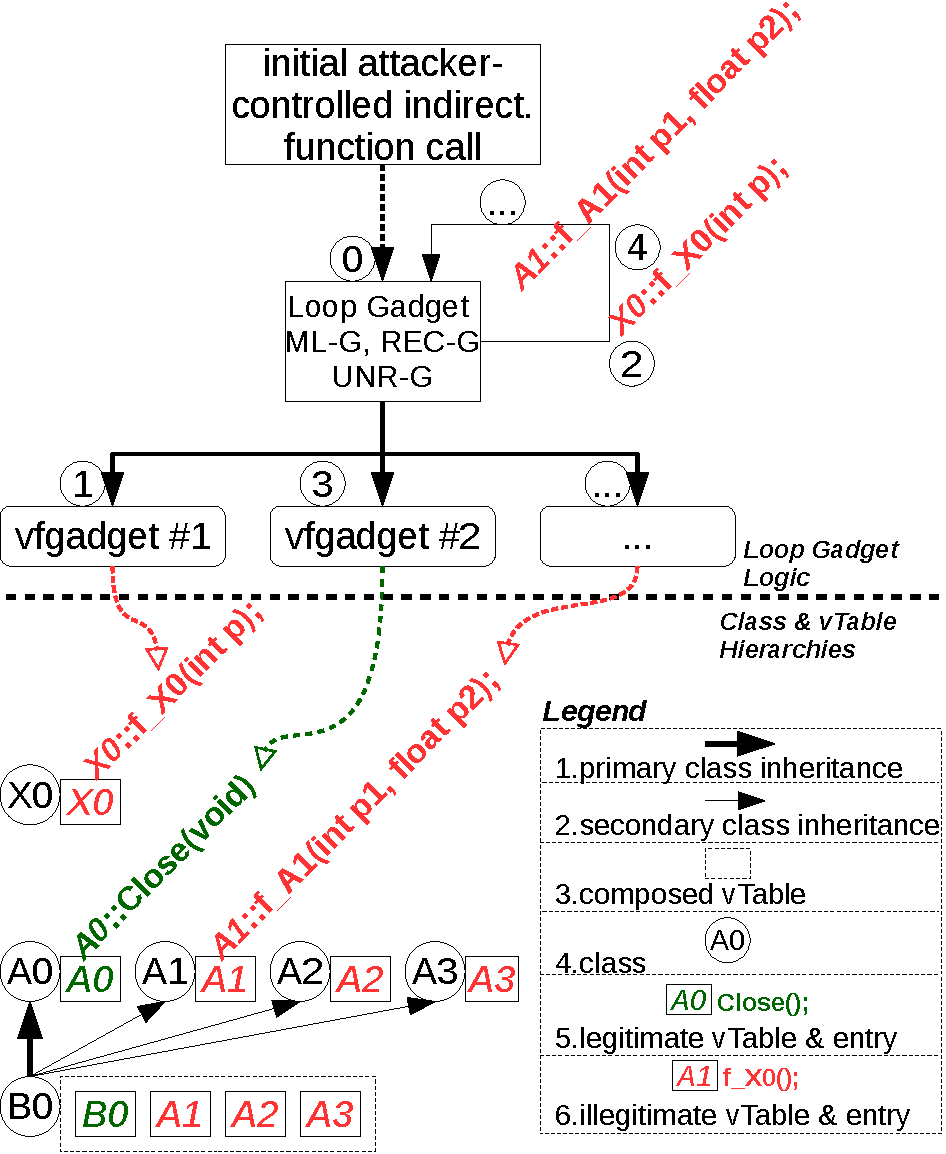
\includegraphics[width=1.3\textwidth]{figures/loop.pdf}
% \end{minipage}
% \caption{Code example used to illustrate how a COOP loop gadget works.}
% \label{Code example used to illustrate how a COOP loop gadget works}
% \end{figure}

%%%%%%%%%%%%%%%%%
 \begin{figure*}[!t]
   \setlength{\unitlength}{0.1\textwidth}
   \begin{picture}(10,4)
   \centering
     \put(6.0,0){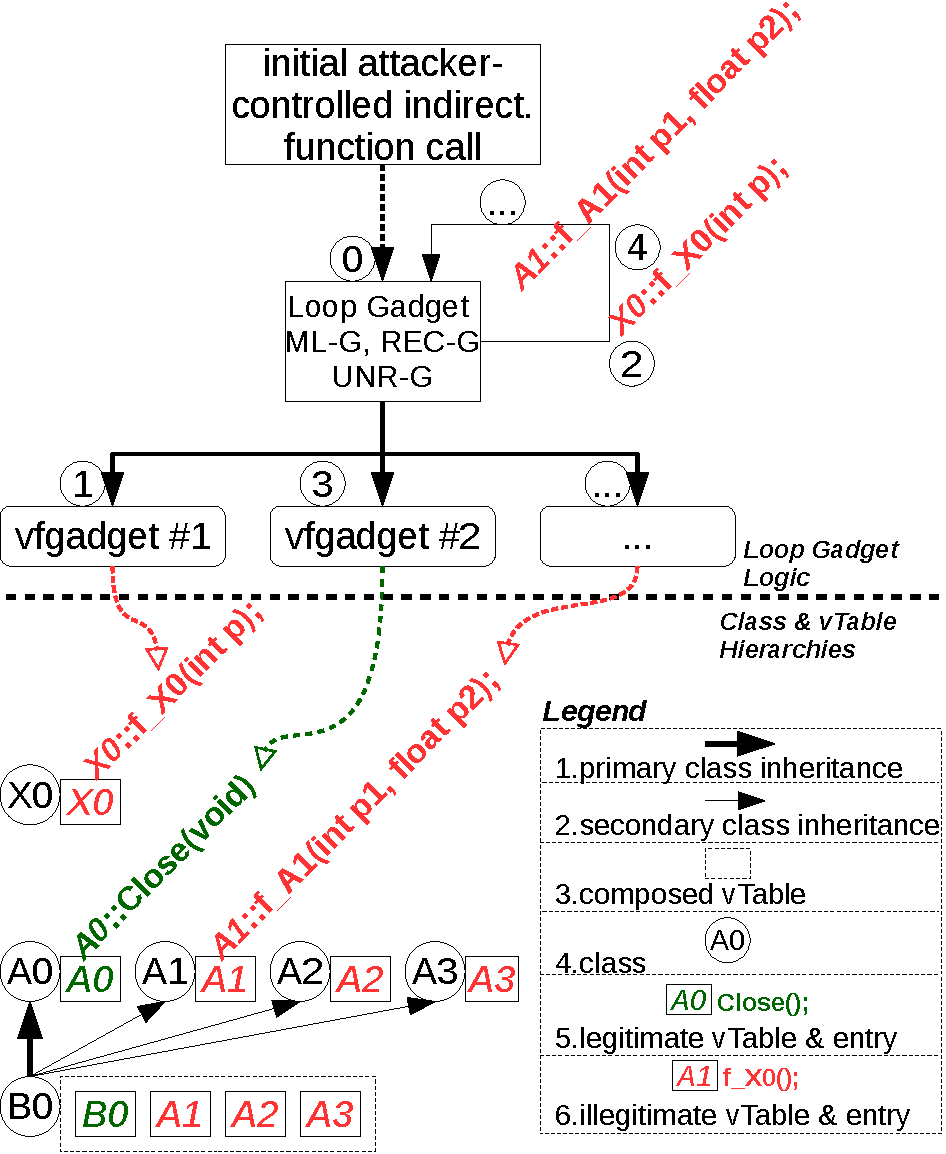
\includegraphics[width=.3\textwidth]{figures/loop.pdf}}
     \put(1.0,2){\usebox{\firstlisting}}
   \end{picture}
\caption{Code presenting how a COOP loop gadget works.}
\label{Code example used to illustrate how a COOP loop gadget works}
\end{figure*}

%the outline is not needed at this moment.
\label{Outline}
\textbf{Outline.} The rest of this paper is organized as follows.
\cref{C++ Bad Forward Indirect Calls} explains forbidden forward indirect calls issues and their security implications.
\cref{chapter:TypeShild Overview} contains a high level overview of \textsc{TypeShield}.
\cref{chapter:Design} describes the theory used and decisions made during the design of \textsc{TypeShield}.
\cref{chapter:Implementation} briefly presents the implementation details of \textsc{TypeShield}.
\cref{chapter:Evaluation} evaluates several properties of \textsc{TypeShield} and
\cref{chapter:Related_Work} surveys related work, respectively.
\cref{chapter:Discussion} contains the discussion, respectively while 
\cref{chapter:Future_Work} highlights future research venues. 
Finally, \cref{chapter:Conclusion} concludes this paper.


